\documentclass[12pt,a4paper]{article}

\usepackage[margin=1in]{geometry}
\usepackage[T1]{fontenc}
\usepackage{lmodern}
\usepackage{graphicx}
\usepackage{booktabs}
\usepackage{array}
\usepackage{tabularx}
\usepackage{float}
\usepackage{amsmath}
\usepackage{enumitem}
\usepackage{setspace}
\usepackage{fancyhdr}
\usepackage[hidelinks]{hyperref}
\usepackage{caption}

\captionsetup{font=small,labelfont=bf}
\setstretch{1.15}
\setlist{itemsep=2pt,topsep=4pt}
\pagestyle{fancy}
\fancyhf{}
\lhead{Smart Fire Detection System}
\rhead{ML Project Report}
\cfoot{\thepage}
\graphicspath{{figures/}}

\begin{document}

% ------------------------------------------------------------------
% Title page
% ------------------------------------------------------------------
\begin{titlepage}
\centering
\vspace*{2cm}
{\Huge\bfseries Smart Fire Detection System\par}
\vspace{0.6cm}
{\Large IoT Sensor and Camera Fusion using Machine Learning\par}
\vspace{1.5cm}
{\large\itshape Machine Learning Project Report\par}
\vspace{3cm}
\begin{tabular}{rl}
\textbf{Name:}        & Your Name \\[4pt]
\textbf{Roll No.:}    & Your Roll Number \\[4pt]
\textbf{Department:}  & Your Department \\[4pt]
\textbf{Institution:} & Your College / University \\[4pt]
\textbf{Guide:}       & Guide Name \\[4pt]
\textbf{Date:}        & \today
\end{tabular}
\vfill
\end{titlepage}

\begin{abstract}
This project builds an early-warning fire detection system that combines two independent sources of evidence: an ESP8266 sensor node (MQ-2 smoke, temperature and humidity) analysed by a Random Forest classifier, and a camera analysed by a YOLO object detector. The two probabilities are merged by weighted late fusion into three alert levels (SAFE, WARNING, ALERT) and displayed live on a React dashboard served by a FastAPI backend. The sensor model was trained on 6{,}633 cleaned readings collected from the hardware. This report describes the data, the machine learning pipeline, the system architecture, the evaluation and the limitations of the work.
\end{abstract}

\tableofcontents
\listoffigures
\listoftables
\newpage

% ------------------------------------------------------------------
\section{Introduction}
Fires are often detected too late when only one cue is used: smoke sensors react to cooking fumes, and cameras can be fooled by lighting. Using both a sensor and a camera lets one cue compensate for the weaknesses of the other.

\subsection{Objectives}
\begin{itemize}
  \item Collect real sensor data from an ESP8266-based hardware node.
  \item Train a classifier that estimates fire risk from MQ-2 smoke, temperature and humidity.
  \item Add a vision model (YOLO) that detects fire and smoke in camera frames.
  \item Fuse both probabilities into a single alert level and show it in real time.
  \item Allow the dashboard to trigger a water pump and servo on the hardware.
\end{itemize}

% ------------------------------------------------------------------
\section{System Architecture}
The system has four layers: edge input (ESP8266 and webcam), a FastAPI backend that runs both models in separate reader threads, a fusion stage, and a React dashboard with actuator control. Figure~\ref{fig:arch} shows the complete runtime architecture.

\begin{figure}[H]
  \centering
  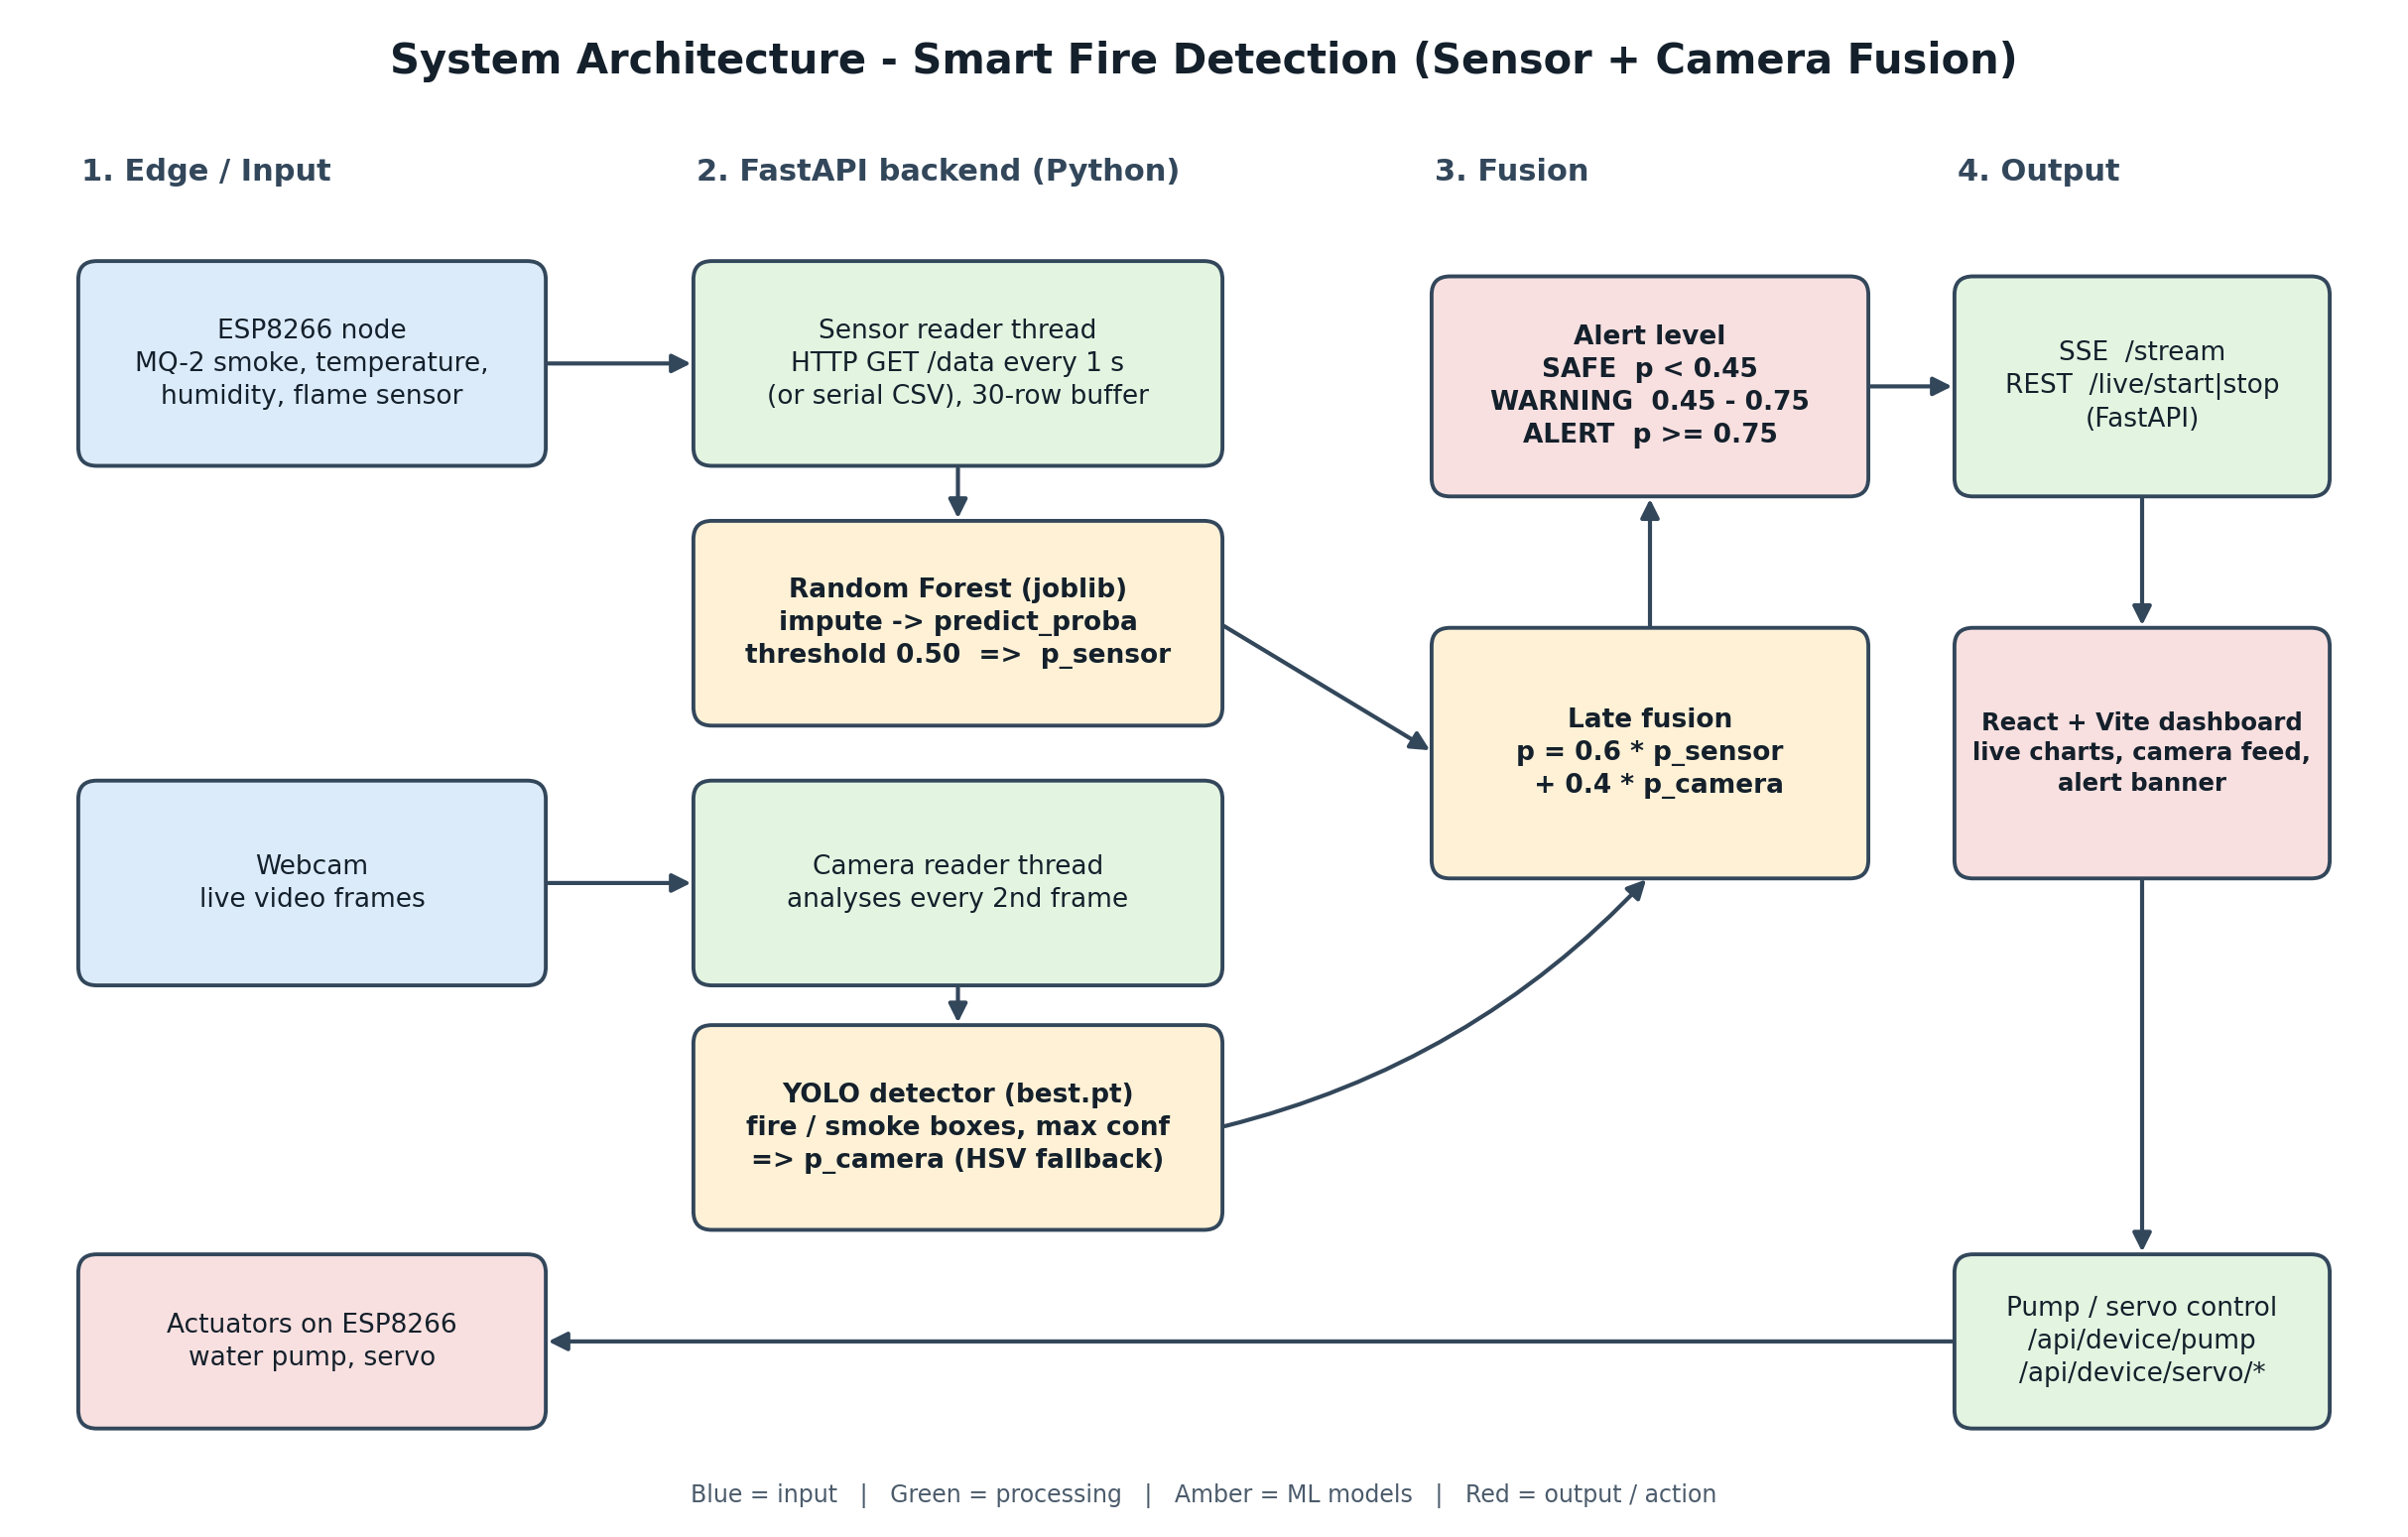
\includegraphics[width=\textwidth]{fig2_system_architecture.png}
  \caption{Runtime system architecture.}
  \label{fig:arch}
\end{figure}

% ------------------------------------------------------------------
\section{Dataset}
Sensor readings were logged from the ESP8266 hardware between 19~November~2025 and 8~January~2026. The raw log holds 7{,}172 rows; after removing invalid or missing rows, 6{,}633 rows remain for modelling (Table~\ref{tab:dataset}).

\begin{table}[H]
\centering
\caption{Summary of the modelling dataset.}
\label{tab:dataset}
\begin{tabularx}{\textwidth}{lX}
\toprule
\textbf{Item} & \textbf{Value} \\
\midrule
Source              & ESP8266 node (MQ-2, MQ-7, temperature/humidity, flame sensor) \\
Rows after cleaning & 6{,}633 \\
Input features      & \texttt{mq2\_smoke}, \texttt{temperature}, \texttt{humidity} \\
Target              & Recorded flame-sensor state (0 = normal, 1 = fire) \\
Class balance       & 5{,}513 negative (83.1\%) / 1{,}120 positive (16.9\%) \\
Feature ranges      & MQ-2: 0--1023 (median 45); temperature: 0--45\,$^{\circ}$C; humidity: 0--99\,\% \\
\bottomrule
\end{tabularx}
\end{table}

The MQ-7 (CO) column was dropped because the deployed hardware does not expose it. The flame sensor is used only to create the label and is deliberately \emph{not} given to the model as an input, since that would leak the answer.

During exploration (notebook \texttt{model/book.ipynb}) other datasets were also examined: an external industrial-hall fire dataset, a Kaggle smoke-detection IoT dataset and an earlier hardware recording with scenarios (normal, smoke puff, smouldering, flame). They informed the choice of features and evaluation design, but the deployed model uses the three-sensor dataset above.

% ------------------------------------------------------------------
\section{Machine Learning Pipeline}
Figure~\ref{fig:pipeline} shows the training pipeline of the sensor model, and Table~\ref{tab:stages} explains each stage.

\begin{figure}[H]
  \centering
  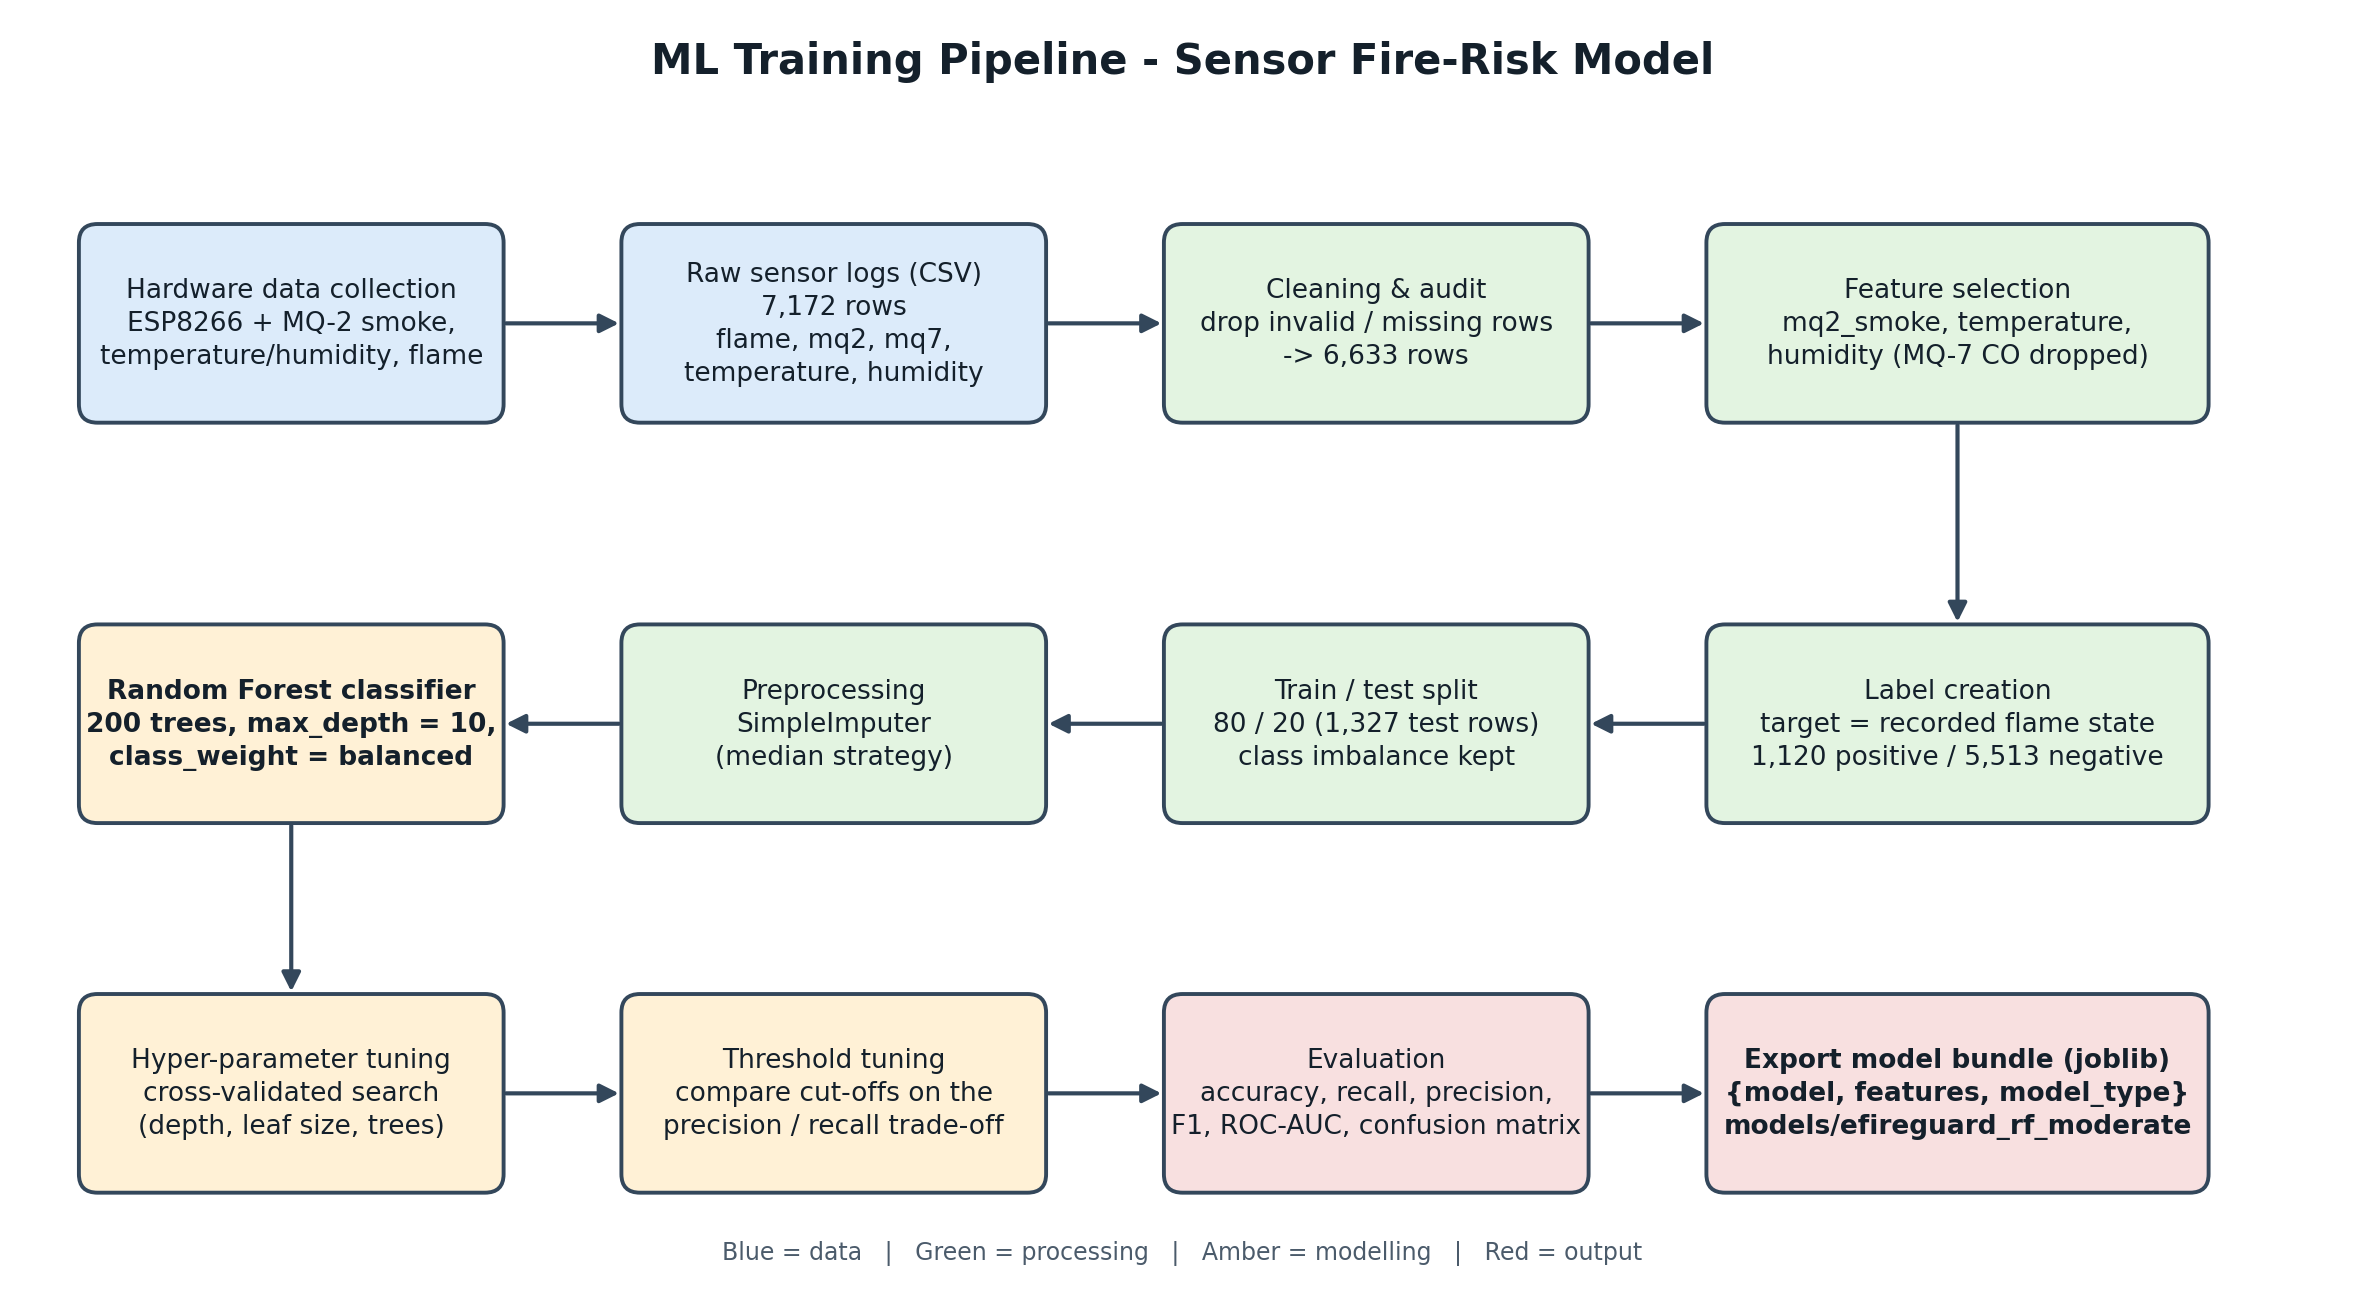
\includegraphics[width=\textwidth]{fig1_ml_pipeline.png}
  \caption{ML training pipeline for the sensor model.}
  \label{fig:pipeline}
\end{figure}

\begin{table}[H]
\centering
\caption{Pipeline stages and rationale.}
\label{tab:stages}
\small
\begin{tabularx}{\textwidth}{l X X}
\toprule
\textbf{Stage} & \textbf{What is done} & \textbf{Why} \\
\midrule
1. Collection        & ESP8266 logs smoke, temperature, humidity and flame state & Real hardware data matches deployment conditions \\
2. Cleaning          & Remove invalid / missing rows; 7{,}172 $\rightarrow$ 6{,}633 & Sensor faults would distort training \\
3. Features / label  & Use three sensors; target = flame state & Only features the live device can supply \\
4. Split             & 80/20 train/test (1{,}327 test rows) & Unseen data for honest evaluation \\
5. Imputation        & \texttt{SimpleImputer}, median strategy & Handles occasional missing readings at inference \\
6. Model             & Random Forest, 200 trees & Robust, non-linear, little scaling needed \\
7. Tuning            & Cross-validated search over depth, leaf size and trees; decision-threshold comparison & Limit overfitting; trade recall against false alarms \\
8. Export            & \texttt{joblib} bundle \{model, features, model\_type\} & Loaded directly by the backend \\
\bottomrule
\end{tabularx}
\end{table}

% ------------------------------------------------------------------
\section{Models}

\subsection{Sensor Model: Random Forest}
The deployed model (\texttt{models/efireguard\_rf\_moderate.joblib}) is a scikit-learn \texttt{Pipeline} consisting of a median \texttt{SimpleImputer} followed by a \texttt{RandomForestClassifier}. A Random Forest averages many decision trees trained on bootstrap samples, which reduces the variance of a single tree. For $T$ trees the predicted fire probability is
\begin{equation}
  p_{\text{sensor}} = \frac{1}{T}\sum_{t=1}^{T} p_t(y = 1 \mid \mathbf{x}),
  \qquad \mathbf{x} = (\text{smoke},\ \text{temperature},\ \text{humidity}).
\end{equation}

\begin{table}[H]
\centering
\caption{Hyper-parameters of the deployed Random Forest.}
\label{tab:hyper}
\begin{tabular}{ll}
\toprule
\textbf{Hyper-parameter} & \textbf{Value} \\
\midrule
\texttt{n\_estimators}                         & 200 \\
\texttt{max\_depth}                            & 10 \\
\texttt{min\_samples\_leaf} / \texttt{min\_samples\_split} & 5 / 10 \\
\texttt{class\_weight}                         & balanced (offsets the 17\% positive class) \\
\texttt{random\_state}                         & 42 \\
Inference threshold (backend)                  & 0.50 on $P(y=1)$, set by \texttt{SENSOR\_THRESHOLD} \\
\bottomrule
\end{tabular}
\end{table}

Other models compared in the notebook included Logistic Regression, Extra Trees, Gradient Boosting and HistGradientBoosting, evaluated with leave-one-session-out cross-validation so that no test session shares data with training.

\subsection{Camera Model: YOLO}
A YOLOv8 detector (initialised from \texttt{yolov8n.pt} and trained with \texttt{camera/train-yolo.py} for up to 50 epochs at 640\,px with early stopping and a small hue-augmentation limit, since colour is the main cue for fire) detects fire and smoke bounding boxes. The highest box confidence in a frame is used as the camera fire probability $p_{\text{camera}}$. If the weights are missing, the backend falls back to an HSV colour heuristic, which is not a reliable detector.

\subsection{Late Fusion and Alert Levels}
The two probabilities are combined as
\begin{equation}
  p_{\text{combined}} = 0.6\,p_{\text{sensor}} + 0.4\,p_{\text{camera}}.
\end{equation}

\begin{table}[H]
\centering
\caption{Alert levels from the combined probability.}
\label{tab:alert}
\begin{tabular}{ll}
\toprule
\textbf{Combined probability} & \textbf{Alert level} \\
\midrule
below 0.45             & SAFE \\
0.45 to below 0.75     & WARNING \\
0.75 and above         & ALERT \\
\bottomrule
\end{tabular}
\end{table}

The sensor is weighted higher because it is a continuous, always-on measurement. The weights and cut-offs are design choices and have not been tuned on a labelled combined dataset.

% ------------------------------------------------------------------
\section{Implementation}
\begin{table}[H]
\centering
\caption{Project components.}
\label{tab:impl}
\small
\begin{tabularx}{\textwidth}{l l X}
\toprule
\textbf{Component} & \textbf{File / folder} & \textbf{Role} \\
\midrule
Exploration and training & \texttt{model/book.ipynb} & Data audit, feature study, model comparison \\
Trained models  & \texttt{models/*.joblib}, \texttt{camera/weights/best.pt} & Sensor Random Forest and YOLO weights \\
Evaluation      & \texttt{evaluation\_below\_90\_v2/} & Metrics, report and CV results of a tuned candidate \\
Backend         & \texttt{backend/api.py} & FastAPI: reader threads, inference, fusion, SSE stream, pump/servo routes \\
Camera tools    & \texttt{camera/} & Dataset checks, YOLO training and evaluation \\
Dashboard       & \texttt{frontend/} (React + Vite) & Live charts, camera feed, alert banner, controls \\
Launcher        & \texttt{start.bat} & Starts backend (port 8000) and frontend (port 5173) \\
\bottomrule
\end{tabularx}
\end{table}

\textbf{Runtime flow.} Every second the backend polls the ESP8266 (\texttt{/data}), appends the reading to a 30-row buffer and runs the Random Forest on the latest row. In parallel the camera thread analyses every second frame with YOLO. Whenever either value updates, the fusion step recomputes the alert level, which is pushed to the dashboard over Server-Sent Events (\texttt{/stream}).

% ------------------------------------------------------------------
\section{Evaluation}
Table~\ref{tab:metrics} is taken from the saved evaluation report (\texttt{evaluation\_below\_90\_v2/evaluation\_report.txt}) for the regularised Random Forest candidate (\texttt{max\_depth}\,=\,3, \texttt{min\_samples\_leaf}\,=\,80, 200 trees) on 1{,}327 held-out rows with decision threshold 0.30.

\begin{table}[H]
\centering
\caption{Test-set metrics of the regularised candidate model.}
\label{tab:metrics}
\begin{tabular}{lc}
\toprule
\textbf{Metric} & \textbf{Value} \\
\midrule
Accuracy                    & 0.892 \\
Balanced accuracy           & 0.869 \\
Precision (fire)            & 0.638 \\
Recall (fire)               & 0.835 \\
Specificity                 & 0.904 \\
F1 score                    & 0.723 \\
ROC-AUC                     & 0.932 \\
Average precision           & 0.798 \\
Matthews corr.\ coefficient & 0.667 \\
\bottomrule
\end{tabular}
\end{table}

\begin{table}[H]
\centering
\caption{Confusion matrix (rows: actual, columns: predicted).}
\label{tab:cm}
\begin{tabular}{lcc}
\toprule
 & \textbf{Predicted normal} & \textbf{Predicted fire} \\
\midrule
\textbf{Actual normal} & 997 (TN) & 106 (FP) \\
\textbf{Actual fire}   & 37 (FN)  & 187 (TP) \\
\bottomrule
\end{tabular}
\end{table}

\textbf{Interpretation.} The model catches about 83\% of fire-state readings and wrongly flags about 10\% of normal readings. A low threshold (0.30) was chosen to favour recall, because a missed fire is more costly than a false alarm. The shallow trees and large leaves keep the model simple, which limits overfitting to repetitive readings.

\emph{Note: these figures belong to the regularised candidate in the evaluation folder. A separate saved evaluation of the deployed model (\texttt{max\_depth}\,=\,10, threshold 0.50) is not included.}

% ------------------------------------------------------------------
\section{Limitations}
\begin{itemize}
  \item The label is the recorded flame-sensor state, so the model predicts what a flame sensor would report from smoke, temperature and humidity. It is a proxy, not independently validated fire detection.
  \item Readings are time-ordered and strongly autocorrelated; a random row split can overestimate accuracy. Splitting by recording session is a stricter test.
  \item Only about 17\% of the data is positive, from one device and environment; generalisation to other rooms and sensors is unproven.
  \item The fusion weights (0.6/0.4) and alert thresholds were chosen by judgement, not optimised.
  \item The camera test set used for quick checks is small, so camera accuracy should not be over-claimed.
  \item The current model uses a single reading; the 30-row buffer is kept for display and future temporal features.
  \item The system is a prototype and must not replace certified fire alarms.
\end{itemize}

% ------------------------------------------------------------------
\section{Conclusion and Future Work}
The project delivers a working end-to-end pipeline: hardware data collection, a Random Forest sensor model, a YOLO camera model, weighted fusion into three alert levels, and a live dashboard with pump and servo control. Future work includes collecting more labelled sessions in varied environments, evaluating with session-wise cross-validation, using rolling-window features from the 30-row buffer, tuning the fusion weights on a combined labelled set, and calibrating probabilities before thresholding.

% ------------------------------------------------------------------
\appendix
\section{Questions to Prepare For}
\begin{table}[H]
\centering
\caption{Likely viva questions.}
\label{tab:qa}
\small
\begin{tabularx}{\textwidth}{>{\raggedright\arraybackslash}p{4.8cm} X}
\toprule
\textbf{Question} & \textbf{Short answer} \\
\midrule
Why Random Forest? & Handles non-linear sensor relationships, robust to noise, little preprocessing, gives probabilities. \\
Why is the flame sensor not an input? & The label comes from it; using it would leak the answer. \\
Why \texttt{class\_weight = balanced}? & Only about 17\% of rows are fire; it stops the model ignoring the minority class. \\
Why a 0.30 threshold in evaluation? & Favours recall: a missed fire costs more than a false alarm. \\
Why fuse sensor and camera? & Independent evidence; each covers the other's failure cases. \\
Why late fusion? & The models are trained separately on different data, so combining probabilities is simplest and robust. \\
Biggest weakness? & Proxy label and a small single-device dataset (Section~8). \\
\bottomrule
\end{tabularx}
\end{table}

\end{document}
